
% License:
% CC BY-NC-SA 3.0 (http://creativecommons.org/licenses/by-nc-sa/3.0/)
%
%%%%%%%%%%%%%%%%%%%%%%%%%%%%%%%%%%%%%%%%%

%----------------------------------------------------------------------------------------
%	PACKAGES AND OTHER DOCUMENT CONFIGURATIONS
%----------------------------------------------------------------------------------------

\documentclass[paper=a4, fontsize=11pt]{scrartcl} % A4 paper and 11pt font size

\usepackage[T1]{fontenc} % Use 8-bit encoding that has 256 glyphs
\usepackage{fourier} % Use the Adobe Utopia font for the document - comment this line to return to the LaTeX default
\usepackage[english]{babel} % English language/hyphenation
\usepackage{amsmath,amsfonts,amsthm} % Math packages
\usepackage{lipsum} % Used for inserting dummy 'Lorem ipsum' text into the template

\usepackage{caption}
\usepackage{subcaption}
\usepackage{graphicx}

\usepackage{float}

\usepackage{blindtext} %for enumarations

\usepackage[]{hyperref}  %link collor

%talbe layout to the right
%\usepackage[labelfont=bf]{caption}
%\captionsetup[table]{labelsep=space,justification=raggedright,singlelinecheck=off}
%\captionsetup[figure]{labelsep=quad}

\usepackage{sectsty} % Allows customizing section commands
\allsectionsfont{\centering \normalfont\scshape} % Make all sections centered, the default font and small caps

\usepackage{fancyhdr} % Custom headers and footers
\pagestyle{fancyplain} % Makes all pages in the document conform to the custom headers and footers
\fancyhead{} % No page header - if you want one, create it in the same way as the footers below
\fancyfoot[L]{} % Empty left footer
\fancyfoot[C]{} % Empty center footer
\fancyfoot[R]{\thepage} % Page numbering for right footer
\renewcommand{\headrulewidth}{0pt} % Remove header underlines
\renewcommand{\footrulewidth}{0pt} % Remove footer underlines
\setlength{\headheight}{13.6pt} % Customize the height of the header

\numberwithin{equation}{section} % Number equations within sections (i.e. 1.1, 1.2, 2.1, 2.2 instead of 1, 2, 3, 4)
\numberwithin{figure}{section} % Number figures within sections (i.e. 1.1, 1.2, 2.1, 2.2 instead of 1, 2, 3, 4)
\numberwithin{table}{section} % Number tables within sections (i.e. 1.1, 1.2, 2.1, 2.2 instead of 1, 2, 3, 4)

%\setlength\parindent{0pt} % Removes all indentation from paragraphs - comment this line for an assignment with lots of text


\setlength\parskip{4pt}

%----------------------------------------------------------------------------------------
%	TITLE SECTION
%----------------------------------------------------------------------------------------

\newcommand{\horrule}[1]{\rule{\linewidth}{#1}} % Create horizontal rule command with 1 argument of height

\title{	
\normalfont \normalsize 
\horrule{0.5pt} \\[0.4cm] % Thin top horizontal rule
\huge  Instruction Fetch DRAC specification version v0.1 \\ % The assignment title
\horrule{2pt} \\[0.5cm] % Thick bottom horizontal rule
}

\author{ Guillem Lopez Paradis} % Your name

\date{\normalsize\today} % Today's date or a custom date

\begin{document}
%\nocite{*}
\maketitle % Print the title

\newpage
\tableofcontents

%----------------------------------------------------------------------------------------
%	Section 1
%----------------------------------------------------------------------------------------

\newpage
\section{General purpose of the module}
\textit{Person in Charge; Guillem Lopez Paradis}

The \textit{Instruction Cache Interface} module is placed in the top module alongside the datapath and the Data Cache Interface.
It is responsible of producing the necessary signals to control the instruction cache.

This module receives signals from the datapath and the response from the instruction cache, and it outputs the following signals:

\begin{itemize}
    \item Request to instruction cache.
    \item Response to the CPU.
\end{itemize}


%----------------------------------------------------------------------------------------
%	Section 2
%----------------------------------------------------------------------------------------

\section{Design placement}
\label{chapter2}

This module has a single instance per core, labeled as rr\_stage\_inst. The instances are always located inside the datapath (datapath.sv) of the core.
RTL for this module is contained in a single file, named regfile.sv. 




\section{Parameters}
\label{chapter3}

All parameters, enums and types used in this module are defined in drac\_pkg or risc\_pkg.

\section{Interface}
\label{chapter 4}

\begin{table}[H]
\centering
\begin{tabular}{llll}
\textbf{Signal name} & \textbf{Width} & \textbf{Type} & \textbf{Description} \\
\hline
clk\_i & 1 & in & Clock \\
rstn\_i & 1 & in & Reset \\
valid\_fetch & 1 & in & The instruction in Fetch is valid \\
id\_cu\_i & struct & in & Signals from Decode stage \\
rr\_cu\_i & struct & in & Signals from Read Register stage \\
exe\_cu\_i & struct & in & Signals from Execution stage \\
wb\_cu\_i & struct & in &  Signals from Write Back stage\\
csr\_cu\_i & struct & in & Signals from the CSRs \\
correct\_branch\_pred\_i & 1 & in & A branch instruction in the Execution \\
 &  &  & stage has been predicted correctly \\

pipeline\_ctrl\_o & struct & out & Signals to stall the stages and to \\
 &  &  & select PC in case of jump \\
pipeline\_flush\_o & struct & out & Signals to flush the stages \\
cu\_if\_o & struct & out & Select next PC: PC, PC+4 or jump \\
invalidate\_icache\_o & 1 & out & Invalidate ICache request \\
invalidate\_buffer\_o & 1 & out & Invalidate the ICache buffer \\
cu\_rr\_o & struct & out & Signals to Read Register stage \\

\end{tabular}
\end{table}


\section{Reset behavior}

This module does not contain reset. Register shall be initialized to 0 by software.

Removing the reset allows mapping memories in srams instead of registers if needed. 






\section{What could not happen}

This module is an interface among modules it is only required to fulfill linting requirements. All signals must match in width with other interfaces. Unused signals shall be removed. 

\section{Behavior}

\subsection{Description of EXE\_STAGE module}

In this section we describe what is the behaviour of exe\_stage when an instruction comes from the datapath at the rising edge of the cycle. All the information is sent inside \emph{from\_rr\_i} signal. 

First step is resolve the bypasses from write back stage. If the instruction coming from write-back is valid, and the field \emph{from\_rr\_i.intr.rs1} equals \emph{from\_wb\_i.rd} then \emph{Data operand 1}. Similar process is done for \emph{Data operand 2}.

In case struct fields \emph{from\_rr\_i.intr.use\_pc} or \emph{from\_rr\_i.intr.use\_imm} are set to 1, \emph{Data operand 1} will be \emph{from\_rr\_i.intr.pc} and \emph{Data operand 2} will be \emph{from\_rr\_i.instr.result}, respectively.

Then the instruction and data operands are feed to all the functional units (Branch Unit, ALU, DIV Unit and MUL Unit). There is a special case in which if \emph{from\_rr\_i.instr.unit} is equal to \emph{UNIT\_MEM}, and \emph{from\_rr\_i.instr.valid} is set to 1, then \emph{req\_cpu\_dcache\_o} is filled the necessary data.

When the functional units finish the requested operation, \emph{to\_wb\_o.result} is filled with the \emph{result\_o} signal of the corresponding functional unit of the instruction. The rest of the signals in \emph{to\_wb\_o} struct are filled with the equivalent signals from the \emph{from\_rr\_i} struct.

The only signals in \emph{to\_wb\_o} that are not directly wired from \emph{from\_rr\_i} are:

\begin{itemize}
    \item \emph{to\_wb\_o.result} mentioned earlier.
    \item \emph{to\_wb\_o.csr\_addr} is the lower 12 bits of \emph{from\_rr\_i.result}, that contains the immediate value.
    \item \emph{to\_wb\_o.ex.valid} contains if the current instruction is rising an exception. It must be set to 1 if there has been an exception in previous stages (\emph{from\_rr\_i.instr.ex.valid} == 1). It must set to 1 if csr\_interrupt\_i is set (CSR has received an interruption), or there has been an exception on dcache (Load or store Misaligned, load or store access fault), or the branch is jumping to a misaligned address. 
    \item \emph{to\_wb\_o.ex.cause} contains what has been the cause of the exception or interruption.
    \item \emph{to\_wb\_o.ex.origin} contains the program counter or address that caused the exception, depending on the cause.
    \item \emph{to\_wb\_o.branch\_taken} is set to 1 if the current branch is a jump or branch and is jumping to the target address.
    \item \emph{to\_wb\_o.result\_pc} contains what should be the program counter of the next instruction.
\end{itemize}

The struct \emph{exe\_if\_branch\_pred\_o} contains all the information about branch prediction at execution stage that must be forwarded to fetch stage. It contains the program counter of the current instruction at execution stage, what is the program counter target computed by the branch, the decision if the branch is taken or not and if the instruction at execution stage is a real branch.

\emph{stall\_o} signal warns control unit that the execution stages needs at least one more cycle to complete the current instruction. It activates when \emph{stall\_o} signal of DIV, MUL or a memory access is set to 1, and the functional unit needed by the instruction matches the module setting the stall.

%--------------------------------------------------------------------------------------------

\subsection{Description of ALU module}

In this section we describe what is the behaviour of ALU module for each of the possible inputs.

\begin{itemize}
  \item ADD: \emph{result\_o} contains the addition of \emph{data\_rs1\_i} plus \emph{data\_rs2\_i} using the standard two's complement notation.
  \item ADDW: \emph{result\_o} contains the addition of \emph{data\_rs1\_i} plus \emph{data\_rs2\_i} using the standard two's complement notation. \emph{result\_o} bits from 63 to 32 must be the sign extension of bit 31.
  \item SUB: \emph{result\_o} contains the subtraction of \emph{data\_rs1\_i} minus \emph{data\_rs2\_i} using the standard two's complement notation.
  \item SUBW: \emph{result\_o} contains the subtraction of \emph{data\_rs1\_i} minus \emph{data\_rs2\_i} using the standard two's complement notation.  \emph{result\_o} bits from 63 to 32 must be the sign extension of bit 31.
  \item SLL: \emph{result\_o} contains the logical left shift of \emph{data\_rs1\_i} by the six lower bits of \emph{data\_rs2\_i}.
  \item SLLW: \emph{result\_o} contains the logical left shift of \emph{data\_rs1\_i} by the five lower bits of \emph{data\_rs2\_i}. \emph{result\_o} bits from 63 to 32 must be the sign extension of bit 31.
  \item SLT: \emph{result\_o} contains 1 if \emph{data\_rs1\_i} < \emph{data\_rs2\_i}, 0  otherwise. < operator uses the standard two's complement notation. 
  \item SLTU: \emph{result\_o} contains 1 if \emph{data\_rs1\_i} < \emph{data\_rs2\_i}, 0  otherwise. < operator uses the standard unsigned notation. 
  \item XOR: \emph{result\_o} contains the bit-wise XOR operation bit-wise \emph{data\_rs1\_i} and \emph{data\_rs2\_i}.
  \item SRL: \emph{result\_o} contains the logical right shift of \emph{data\_rs1\_i} by the six lower bits of \emph{data\_rs2\_i}.
  \item SRLW: \emph{result\_o} contains the logical right shift of \emph{data\_rs1\_i} by the five lower bits of \emph{data\_rs2\_i}. \emph{result\_o} bits from 63 to 32 must be the sign extension of bit 31.
  \item SRA: \emph{result\_o} contains the arithmetic right shift of \emph{data\_rs1\_i} by the six lower bits of \emph{data\_rs2\_i}.
  \item SRAW: \emph{result\_o} contains the arithmetic right shift of \emph{data\_rs1\_i} by the five lower bits of \emph{data\_rs2\_i}. \emph{result\_o} bits from 63 to 32 must be the sign extension of bit 31.
  \item OR:  \emph{result\_o} contains the bit-wise OR operation bit-wise \emph{data\_rs1\_i} and \emph{data\_rs2\_i}.
  \item AND: \emph{result\_o} contains the bit-wise AND operation bit-wise \emph{data\_rs1\_i} and \emph{data\_rs2\_i}.
\end{itemize}

\subsubsection{Examples}

In the following example we can see three consecutive operations in the ALU module. In first cycle the ALU performs an ADD operation, in the second cycle does a SLL, and in the third cycle ALU computes a bit-wise OR. ALU returns always the result on the same cycle

\begin{figure}[h]
\centering
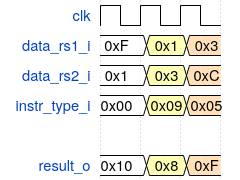
\includegraphics[width=8cm]{wave_alu.png}
\end{figure}

%---------------------------------------------------------------------------------------------

\subsection{Description of Branch Unit module}

In this section we describe what is the behaviour of BU module for each of the possible inputs.

\begin{itemize}
  \item JAL: \emph{link\_pc\_o} contains the addition of \emph{pc\_i} plus \emph{0x4}, \emph{taken\_o} is \textbf{always} equal to \\ \emph{PRED\_NOT\_TAKEN}.
  \item JALR: \emph{link\_pc\_o} and \emph{result\_o} contain the addition of \emph{pc\_i} plus \emph{0x4}, \emph{taken\_o} is \textbf{always} equal to \emph{PRED\_TAKEN}.
  \item BEQ: \emph{taken\_o} is equal to \emph{PRED\_TAKEN} if \emph{data\_rs1\_i} is \textbf{equal} to \emph{data\_rs2\_i}. Signal \emph{result\_o} is equal to \emph{pc\_i} plus  \emph{imm\_i} if \emph{taken\_o} is equal to \emph{PRED\_TAKEN}, otherwise \emph{result\_o} is equal to \emph{pc\_i} plus \emph{0x4}.
  \item BNE: \emph{taken\_o} is equal to \emph{PRED\_TAKEN} if \emph{data\_rs1\_i} is \textbf{not} equal to \emph{data\_rs2\_i}. Signal \emph{result\_o} is equal to \emph{pc\_i} plus  \emph{imm\_i} if \emph{taken\_o} is equal to \emph{PRED\_TAKEN}, otherwise \emph{result\_o} is equal to \emph{pc\_i} plus \emph{0x4}.
  \item BLT: \emph{taken\_o} is equal to \emph{PRED\_TAKEN} if \emph{data\_rs1\_i} is \textbf{lower} than \emph{data\_rs2\_i}. Lower refers to signed comparison in two’s complement notation . Signal \emph{result\_o} is equal to \emph{pc\_i} plus  \emph{imm\_i} if \emph{taken\_o} is equal to \emph{PRED\_TAKEN}, otherwise \emph{result\_o} is equal to \emph{pc\_i} plus \emph{0x4}.
  \item BGE: \emph{taken\_o} is equal to \emph{PRED\_TAKEN} if \emph{data\_rs1\_i} is \textbf{not lower} than \emph{data\_rs2\_i}. Lower refers to signed comparison in two’s complement notation . Signal \emph{result\_o} is equal to \emph{pc\_i} plus  \emph{imm\_i} if \emph{taken\_o} is equal to \emph{PRED\_TAKEN}, otherwise \emph{result\_o} is equal to \emph{pc\_i} plus \emph{0x4}.
  \item BLTU: \emph{taken\_o} is equal to \emph{PRED\_TAKEN} if \emph{data\_rs1\_i} is \textbf{lower} than \emph{data\_rs2\_i}. Lower refers to \textbf{unsigned representation}. Signal \emph{result\_o} is equal to \emph{pc\_i} plus  \emph{imm\_i} if \emph{taken\_o} is equal to \emph{PRED\_TAKEN}, otherwise \emph{result\_o} is equal to \emph{pc\_i} plus \emph{0x4}.
  \item BGEU: \emph{taken\_o} is equal to \emph{PRED\_TAKEN} if \emph{data\_rs1\_i} is \textbf{not lower} than \emph{data\_rs2\_i}. Lower refers to \textbf{unsigned representation}. Signal \emph{result\_o} is equal to \emph{pc\_i} plus  \emph{imm\_i} if \emph{taken\_o} is equal to \emph{PRED\_TAKEN}, otherwise \emph{result\_o} is equal to \emph{pc\_i} plus \emph{0x4}.
\end{itemize}

\subsubsection{Examples}

In the following example we can see three consecutive operations in the Branch Unit module. In first cycle the an BEQ operation, in the second cycle does a BNE, and in the third cycle JALR.  Branch Unit returns always the result on the same cycle

\begin{figure}[h]
\centering
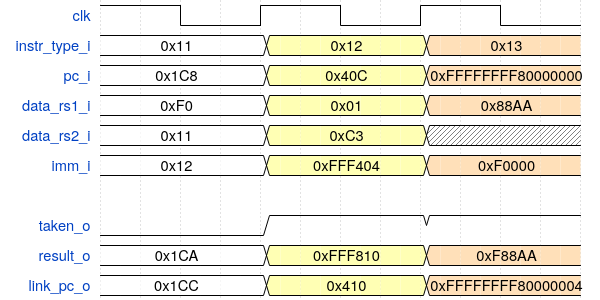
\includegraphics[width=1\linewidth]{wave_branch_unit.png}
\end{figure}


\section{Special cases, corner cases}
Some comments have already been made about special and corner cases such as exceptions, not supported instructions and some non-used bits on some instructions.



\end{document}